\documentclass[11pt,a4paper,titlepage]{article}
\usepackage[a4paper]{geometry}
\usepackage[utf8]{inputenc}
\usepackage[english]{babel}
\usepackage{lipsum}
\usepackage{eurosym}
\usepackage{rotating}

\usepackage{amsmath, amssymb, amsfonts, amsthm, mathtools}
% mathtools for: Aboxed (put box on last equation in align environment)
\usepackage{microtype} %improves the spacing between words and letters

\usepackage{lipsum}
\usepackage{threeparttable}
\usepackage{tabularx}
\usepackage{multirow}
\usepackage{booktabs}
\newcommand{\tabitem}{~~\llap{\textbullet}~~}
\usepackage{graphicx}
\graphicspath{ {./figures/} {./eps/}}
\usepackage{epsfig}
\usepackage{epstopdf}
\usepackage{verbatim}
\usepackage{textcomp}
\usepackage{tikz}
\usetikzlibrary{shapes,arrows}

%%%%%%%%%%%%%%%%%%%%%%%%%%%%%%%%%%%%%%%%%%%%%%%%%%
%% COLOR DEFINITIONS
%%%%%%%%%%%%%%%%%%%%%%%%%%%%%%%%%%%%%%%%%%%%%%%%%%
 % Enabling mixing colors and color's call by 'svgnames'
%%%%%%%%%%%%%%%%%%%%%%%%%%%%%%%%%%%%%%%%%%%%%%%%%%
\definecolor{MyColor1}{HTML}{CC0000} %mix personal color
\newcommand{\textb}{\color{Black} \usefont{OT1}{lmss}{m}{n}}
\newcommand{\blue}{\color{MyColor1} \usefont{OT1}{lmss}{m}{n}}
\newcommand{\blueb}{\color{MyColor1} \usefont{OT1}{lmss}{b}{n}}
\newcommand{\red}{\color{LightCoral} \usefont{OT1}{lmss}{m}{n}}
\newcommand{\green}{\color{Turquoise} \usefont{OT1}{lmss}{m}{n}}
%%%%%%%%%%%%%%%%%%%%%%%%%%%%%%%%%%%%%%%%%%%%%%%%%%


%%%%%%%%%%%%%%%%%%%%%%%%%%%%%%%%%%%%%%%%%%%%%%%%%%
%% FONTS AND COLORS
%%%%%%%%%%%%%%%%%%%%%%%%%%%%%%%%%%%%%%%%%%%%%%%%%%
%		SECTIONS
%%%%%%%%%%%%%%%%%%%%%%%%%%%%%%%%%%%%%%%%%%%%%%%%%%
\usepackage{titlesec}
\usepackage{sectsty}
%%%%%%%%%%%%%%%%%%%%%%%%
%set section/subsections HEADINGS font and color
\sectionfont{\color{MyColor1}}  % sets colour of sections
\subsectionfont{\color{MyColor1}}  % sets colour of sections

%set section enumerator to arabic number (see footnotes markings alternatives)
\renewcommand\thesection{\arabic{section}.} %define sections numbering
\renewcommand\thesubsection{\thesection\arabic{subsection}} %subsec.num.

%define new section style
\newcommand{\mysection}{
\titleformat{\section} [runin] {\usefont{OT1}{lmss}{b}{n}\color{MyColor1}}
{\thesection} {3pt} {} }

%%%%%%%%%%%%%%%%%%%%%%%%%%%%%%%%%%%%%%%%%%%%%%%%%%
%		CAPTIONS
%%%%%%%%%%%%%%%%%%%%%%%%%%%%%%%%%%%%%%%%%%%%%%%%%%
\usepackage{caption}
\usepackage{subcaption}
%%%%%%%%%%%%%%%%%%%%%%%%
\captionsetup[figure]{labelfont={color=MyColor1}}

%%%%%%%%%%%%%%%%%%%%%%%%%%%%%%%%%%%%%%%%%%%%%%%%%%
%		!!!EQUATION (ARRAY) --> USING ALIGN INSTEAD
%%%%%%%%%%%%%%%%%%%%%%%%%%%%%%%%%%%%%%%%%%%%%%%%%%
%using amsmath package to redefine eq. numeration (1.1, 1.2, ...)
%%%%%%%%%%%%%%%%%%%%%%%%
\renewcommand{\theequation}{\thesection\arabic{equation}}

%set box background to grey in align environment
\usepackage{etoolbox}% http://ctan.org/pkg/etoolbox
\makeatletter
\patchcmd{\@Aboxed}{\boxed{#1#2}}{\colorbox{black!15}{$#1#2$}}{}{}%
\patchcmd{\@boxed}{\boxed{#1#2}}{\colorbox{black!15}{$#1#2$}}{}{}%
\makeatother
%%%%%%%%%%%%%%%%%%%%%%%%%%%%%%%%%%%%%%%%%%%%%%%%%%

\newcommand{\DP}[1]{\textcolor{blue}{\textbf{(DP says: #1)}}}
\newcommand{\cri}[1]{\textcolor{green}{\textbf{(Cri says: #1)}}}

\makeatletter
\let\reftagform@=\tagform@
\def\tagform@#1{\maketag@@@{(\ignorespaces\textcolor{red}{#1}\unskip\@@italiccorr)}}
\renewcommand{\eqref}[1]{\textup{\reftagform@{\ref{#1}}}}
\makeatother
\usepackage[hidelinks]{hyperref}

%% LISTS CONFIGURATION %%
\usepackage{enumitem}
\setlist[enumerate,1]{start=0}
\renewcommand{\labelenumii}{\theenumii}
\renewcommand{\theenumii}{\theenumi.\arabic{enumii}.}

\usepackage[acronym]{glossaries}
\newacronym{pmu}{PMU}{Power Management Unit}
\newacronym{pcb}{PCB}{Printed Circuit Board}
\newacronym{ic}{IC}{Integrated Circuit}
\newacronym{emc}{EMC}{Electromagnetic compatibility}
\newacronym{smd}{SMD}{Surface Mounted Device}

%%%%%%%%%%%%%%%%%%%%%%%%%%%%%%%%%%%%%%%%%%%%%%%%%%
%% PREPARE TITLE
%%%%%%%%%%%%%%%%%%%%%%%%%%%%%%%%%%%%%%%%%%%%%%%%%%
\title{\blue User equipment and terminals \\
\blueb Wii U power and design analysis}
\author{Davide Peron\\ Cristina Gava}
\date{\today}
%%%%%%%%%%%%%%%%%%%%%%%%%%%%%%%%%%%%%%%%%%%%%%%%%%

\begin{document}
\maketitle

\tableofcontents
\clearpage

\section{Power supply}
  \subsection{Wii U main console}
		  On the Wii U motherboard there is a discrete number of components involved in the power supply section, there are both passive components, discrete semiconductors and \glspl{ic} all working together to power the \gls{pcb}. In \autoref{tab:power} we summarized the main components listed under type and name: we can see the huge amount of passive components needed to support the integrated circuits and the discrete amount of transistors and		  diodes; on the other hand the number of integrated circuit is restrained.

		  In \autoref{fig:motherboard} a photo of the motherboard section regarding the power supply is shown: the red squares represent three N-channel MOSFET, used to minimize losses in power conversion. Since one of their applications is for a regulator in DC/DC converter, we suppose they are part of the power supply system in the board \cite{mosfet8026}.

		  \begin{figure}
				\centering
				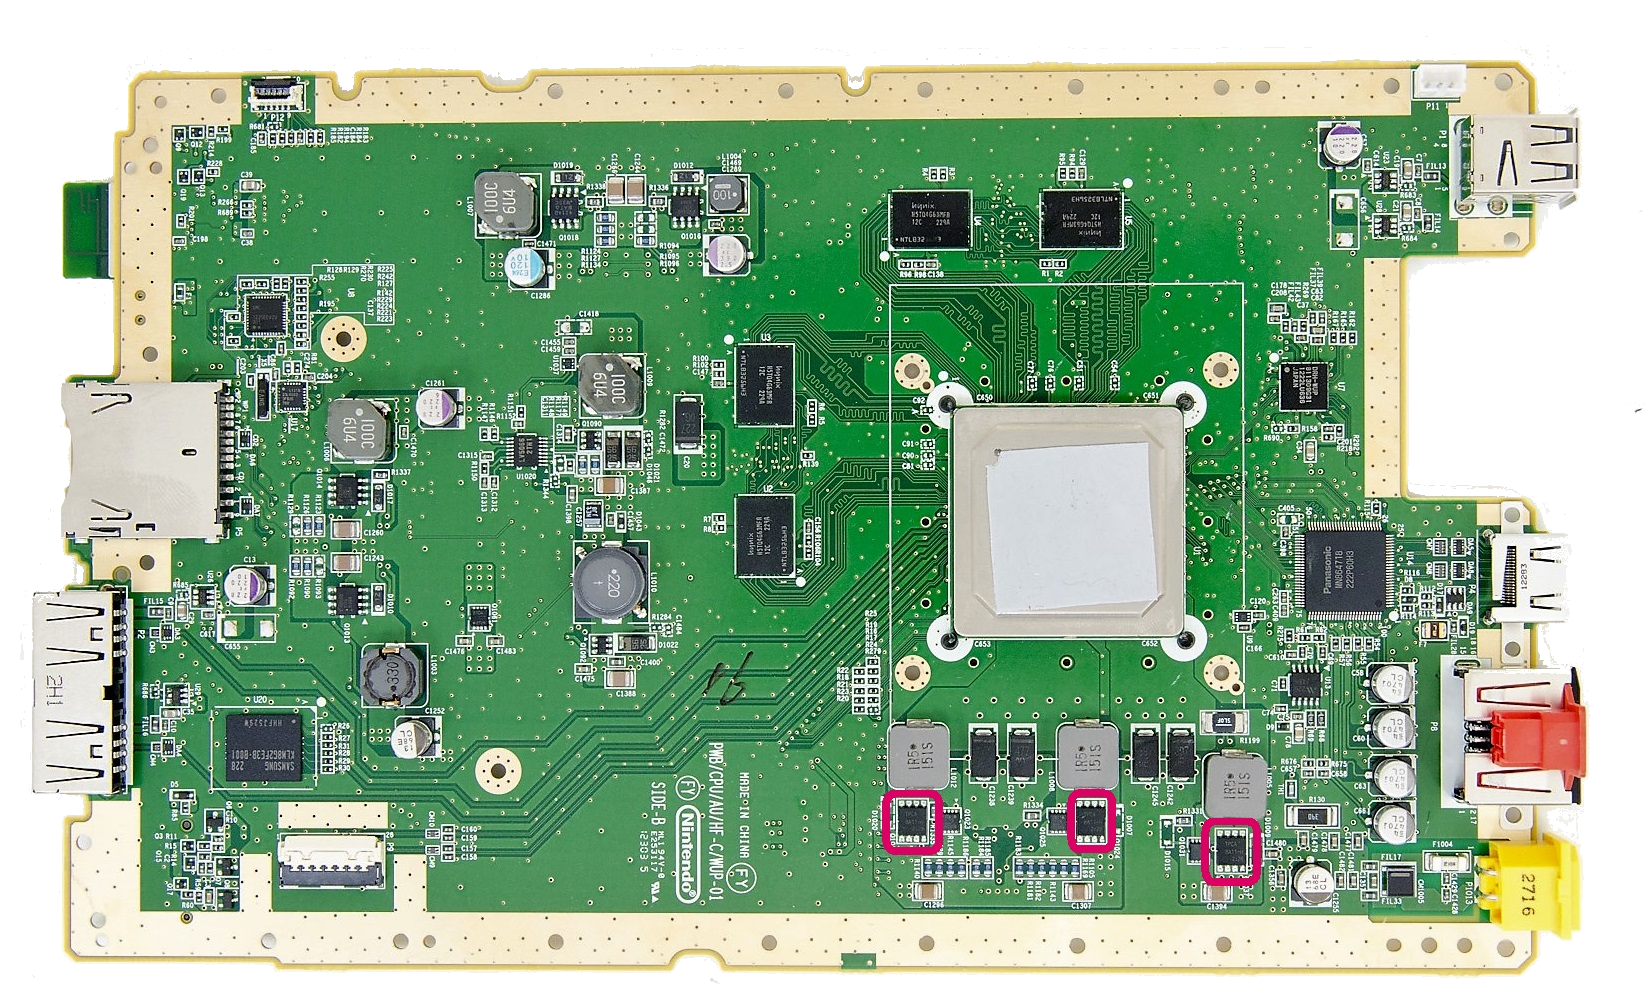
\includegraphics[width = .85\textwidth]{motherboard_front.png}
				\caption{Motherboard front part (power section)}
				\label{fig:motherboard}
		  \end{figure}

		  \subsubsection{Integrated circuits description}
				The three main integrated components that are worth to be described are:
				\begin{itemize}
				  \item \textit{The power management \gls{ic}}, model TPS65070RSL from Texas Instruments;
				  \item \textit{The Regulator DC/DC Converter, Step-Up}, model AIC1634GG from Analog Integration corp.;
				  \item \textit{The switching Regulator DC/DC Controller, Step-Down}, model LV5066V from ON Semiconductors.
				\end{itemize}

				\begin{figure}
				  \begin{minipage}{.5\textwidth}
				  \centering
				  \begin{tabular}{llr}
				  \toprule
				  \textbf{Component type} & \textbf{Name} & \textbf{Qty}\\
				  \midrule
				  Integrated circuit & & \\
				   & Regulator & 7\\
				   & Analog IC & 5\\
				   & Voltage Detector & 1\\
				   & Power Manag. IC & 1\\
				  \hline
				  Discrete Semiconductor & &\\
				   & Diode & 30\\
				   & Transistor & 35\\
				  \hline
				  Passive comp. & &\\
				   & Capacitor & 176\\
				   & Fuse & 1\\
				   & Ferrite Bead & 6\\
				   & Inductor & 16\\
				   & Resistor & 148\\
				  \bottomrule
				  \end{tabular}
				  \caption{Power supply component list}
				  \label{tab:power}
				  \end{minipage}
					\begin{minipage}{.5\textwidth}
				  \centering
				  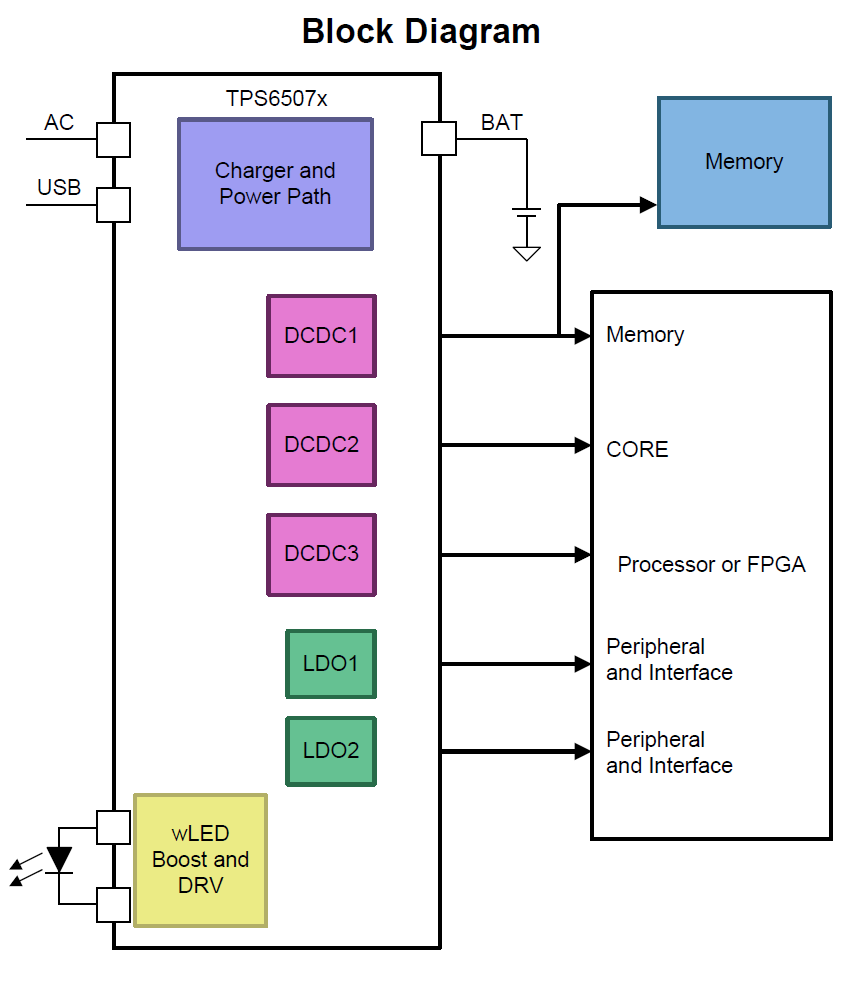
\includegraphics[width = .9\textwidth]{power_managIC.png}
				  \caption{Schematic for TPS65070RSL}
				  \label{fig:TPS65070RSL}
				  \end{minipage}
				\end{figure}

				\begin{description}
				  \item [Control power \gls{ic} TPS65070RSL] Is a single chip power solution for portable applications that can be powered through a USB port or directly by a DC voltage from a wall adapter connected to \textquotedblleft AC\textquotedblright\ pin. The module has the following main characteristics:
						\begin{itemize}
							\item 2A output current on the power path;
							\item Thermal regulation;
							\item 3 Step-down converters
								\begin{itemize}
									\item Fixed-frequency operation at 2.25 MHZ;
									\item Up to 1.5 A output current;
									\item Adjustable or fixed output Voltage;
									\item $2.8V < V_{IN} < 6.3V$
									\item $19\mu A$ of quiescent current per converter;
									\item 100\% Duty cycle for lowest dropout;
								\end{itemize}
						\end{itemize}
				  A block diagram of the module is represented in \autoref{fig:TPS65070RSL}.

				  The two inputs to the power path (AC and USB) support the same voltage rating but normally have different current limits (Ac is at the higher limit). If voltage is applied at both inputs and both are enabled AC will be preferred over USB and the device will only be powered from AC. The current at the input is shared between charging the battery and powering the system load; anyway priority is given to the system load. The current is always monitored so that if the sum of the charging and
				  system load currents exceeds the present maximum input current the charging current is reduced automatically \cite{ICpower}.

				  \item[The Regulator DC/DC Converter AIC1634GG] The module is a current-mode pulse-width modulation (PWM), step-up DC/DC Converter which, through the N-channel MOSFET, allows for step-up applications with up to 30V output voltage. The high switching frequency (1.4MHz) allows the use of small external components.

				  There are several characteristics that can be compared in the module, here we list just two comparisons as examples. The first chart (\autoref{fig:efficiency}), shows how the efficiency of the module varies with the evolution of the output current: it can be seen that its value rapidly saturates for low current values and starts decreasing beyond the 40 mA threshold. The second chart (\autoref{fig:SwFreq}) describes the evolution of the switching frequency over the temperature: differently from the efficiency, the frequency continues to constantly grow with the temperature increase \cite{stepupConv}.

				  \autoref{fig:blocchi} shows the block diagram for the module.

				  \begin{figure}
						\begin{minipage}{.5\textwidth}
						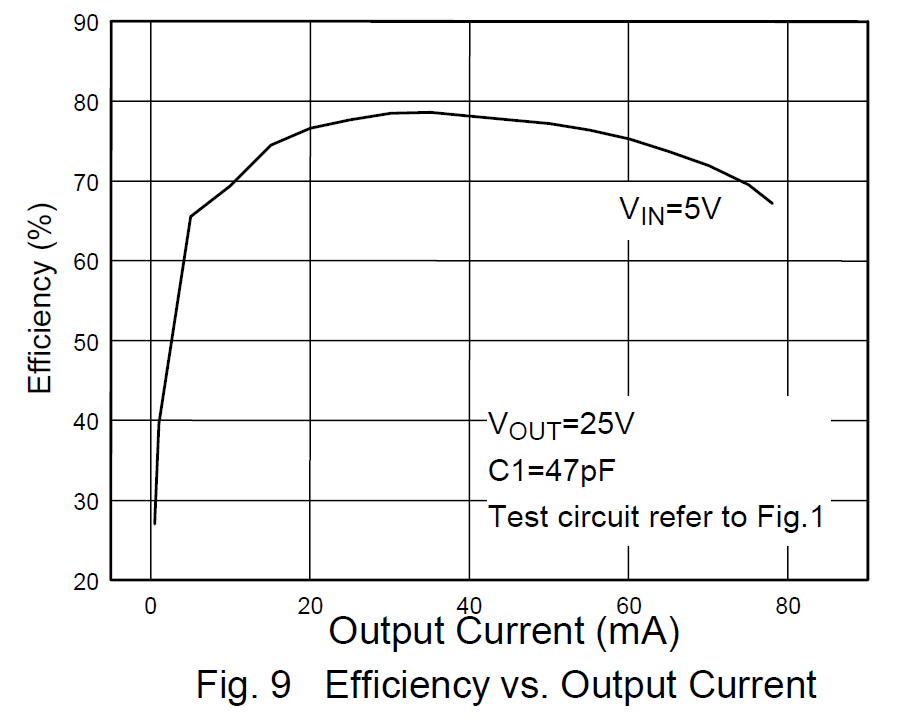
\includegraphics[width = \textwidth]{efficiencyVScurrent.png}
						\caption{}
						\label{fig:efficiency}
						\end{minipage}
						\hspace{5mm}
						\begin{minipage}{.5\textwidth}
						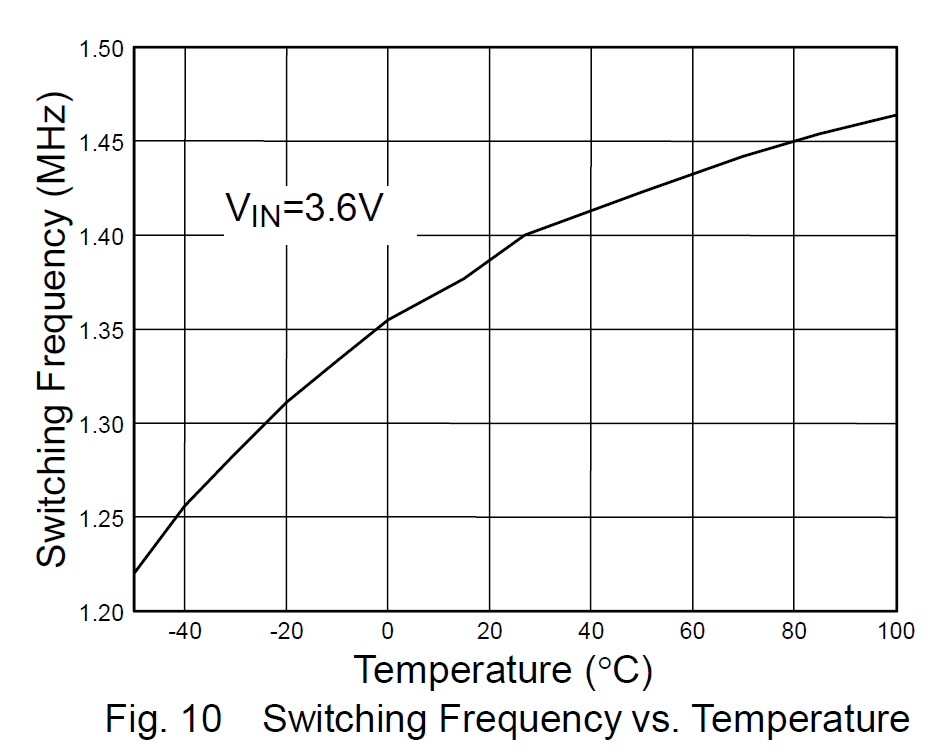
\includegraphics[width = \textwidth]{frequencyVStemp.png}
						\caption{}
						\label{fig:SwFreq}
						\end{minipage}
				  \end{figure}

					\begin{figure}[h]
						\begin{minipage}{.55\textwidth}
							\centering
							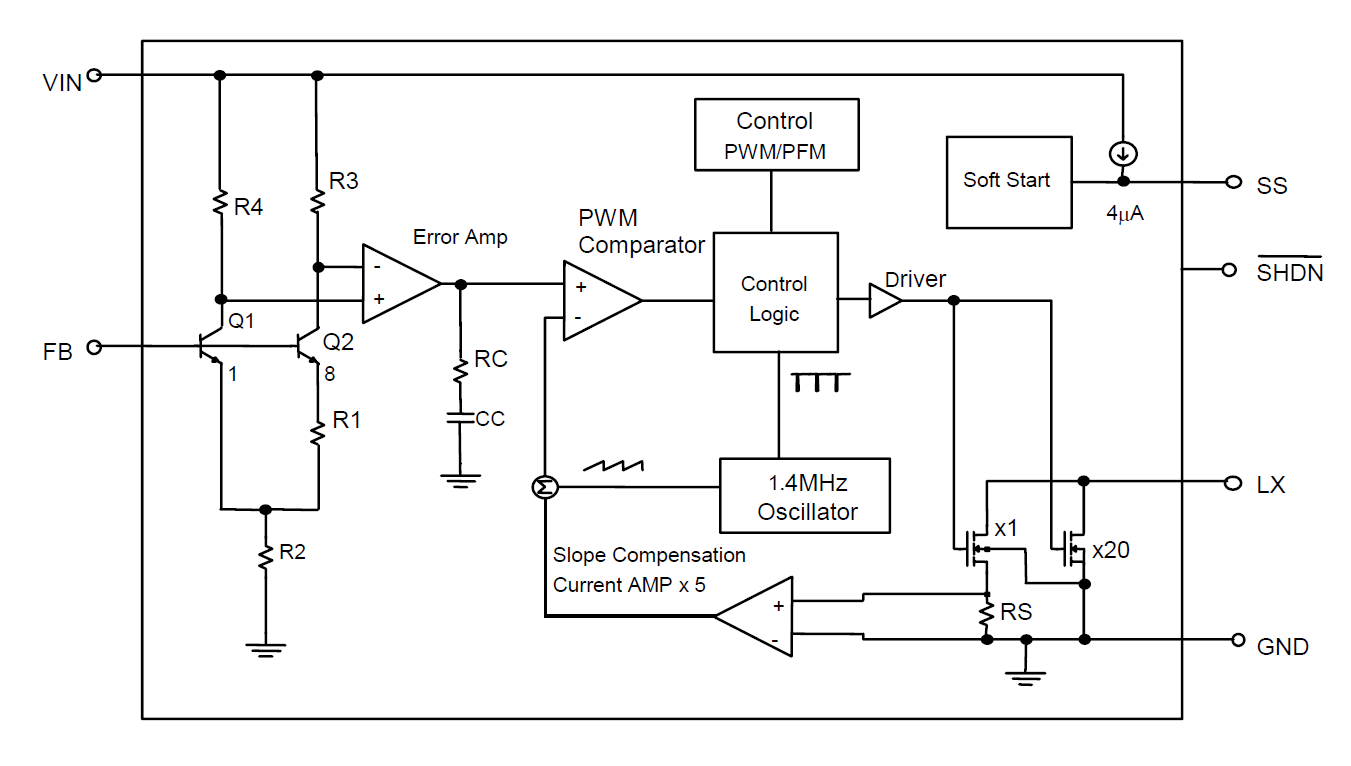
\includegraphics[width = \textwidth]{Schema_blocchi_stepup.png}
							\caption{AIC1634GG block diagram}
							\label{fig:blocchi}
						\end{minipage}
						\hspace{5mm}
						\begin{minipage}{.45\textwidth}
							\centering
							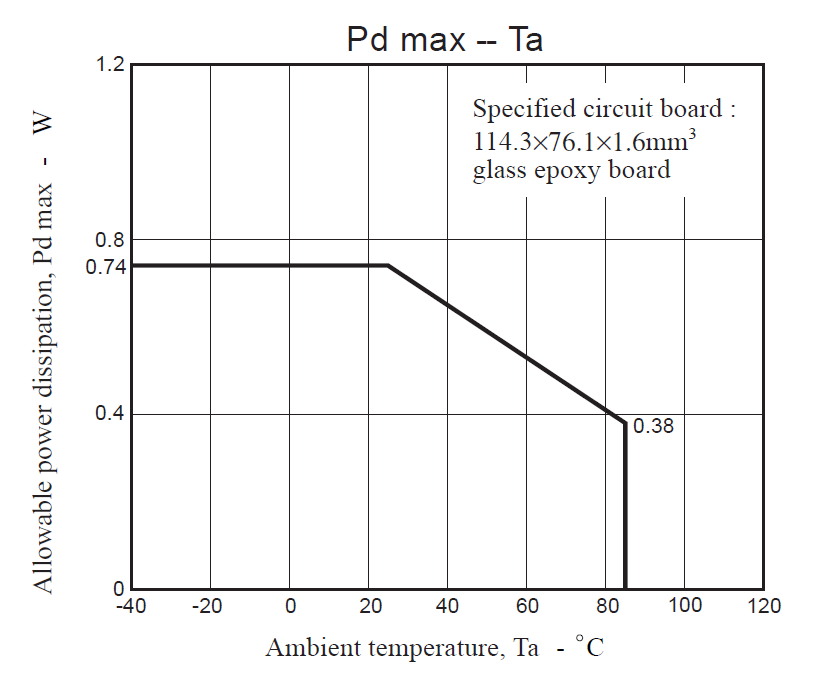
\includegraphics[width = .95\textwidth]{powerVStemp.png}
							\caption{Power constraint over the ambient temperature}
							\label{fig:pdmax}
						\end{minipage}
					\end{figure}

				  \item[The switching Regulator DC/DC Controller LV5066V] The last element of this analysis is a step-down switching regulator controller: it has one channel with an operation current of 80$\mu A$ and low power consumption. Also, from \autoref{fig:pdmax} it can be observed the evolution of the allowable power dissipation depending on the ambient temperature: it can be seen how there is a clear power constraint, with a linear decrement of the latter during the interval representing the normal temperature range of a room.

				\end{description}

\section{Power Management} \label{sec:power_management}
	\subsection{Wii U}
		The Wii U transformer has a maximum output voltage of 15V and a maximum output current of 5A, so this console consumes $15\cdot 5 = 75W$ while under full load. Actually, even when a resources demanding game is running, the power consumed by Wii U is a bit more than an half of the maximum power consumption.
		\begin{figure}[htbp]
			\centering
			\begin{minipage}{0.45\textwidth}
				\centering
				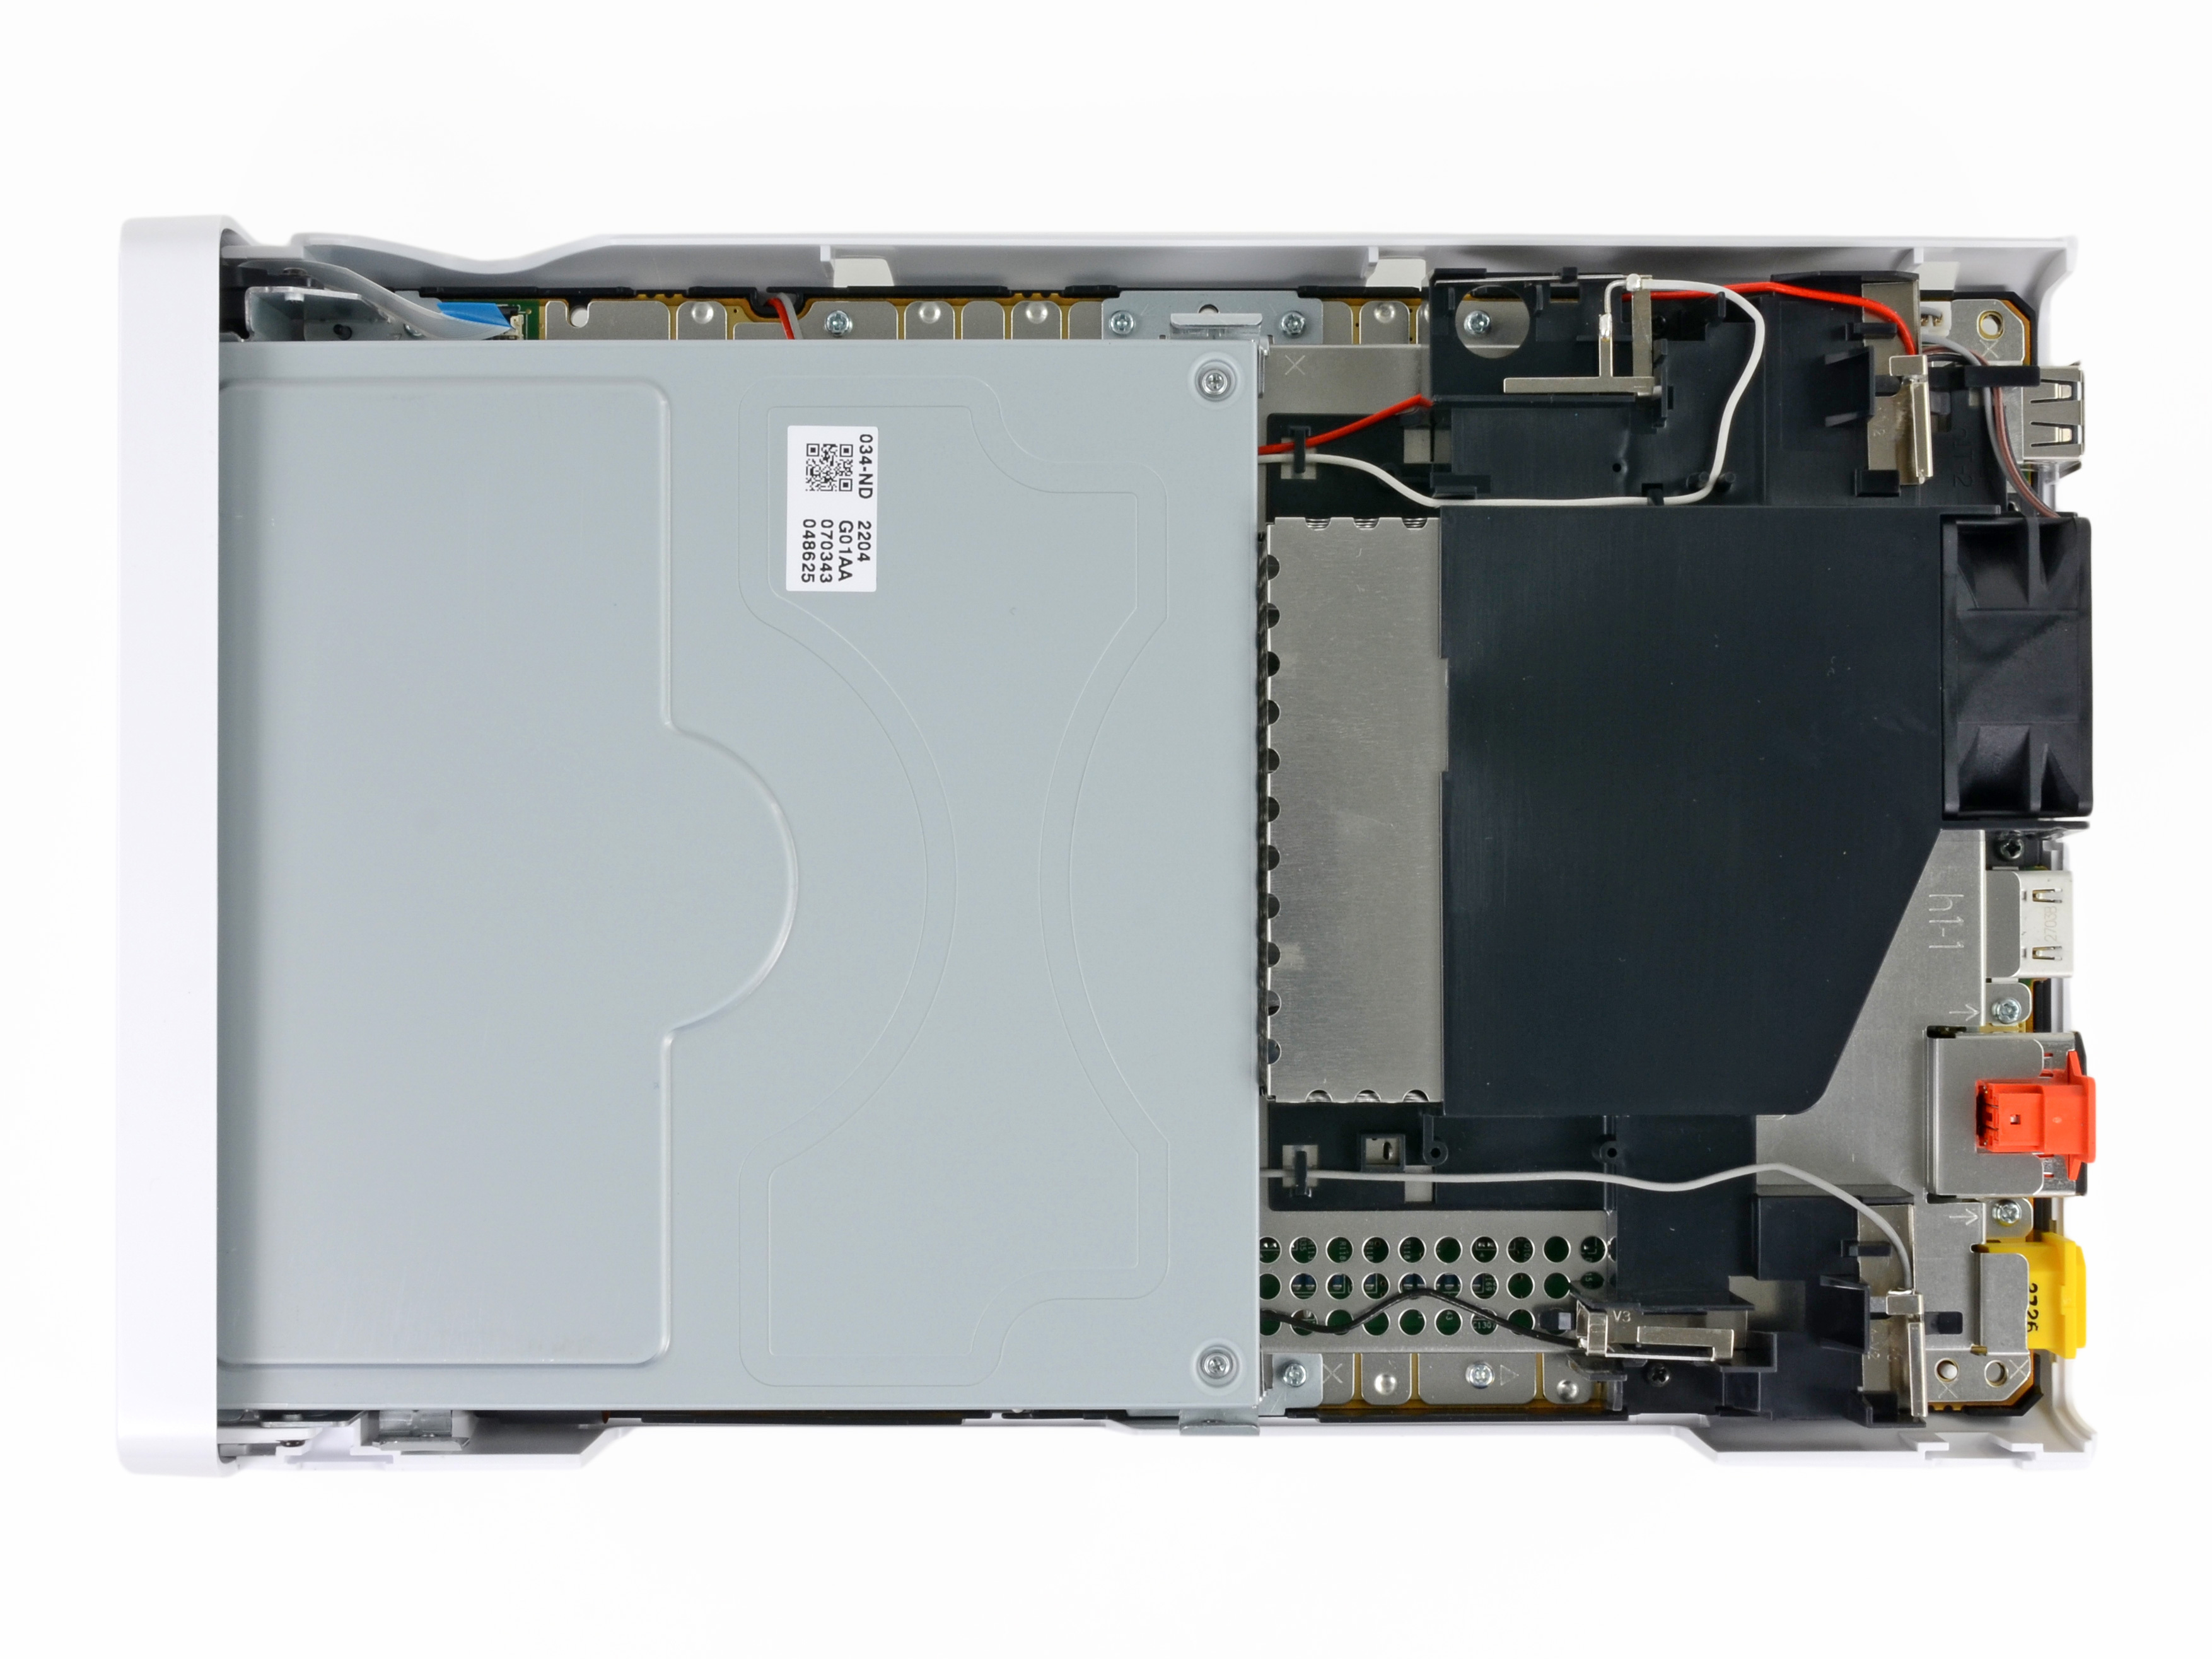
\includegraphics[width=\textwidth]{external_view.jpeg}
				\caption{Wii U without external case}
				\label{fig:external}
			\end{minipage}
			\hspace{0.5cm}
			\begin{minipage}{0.45\textwidth}
				\centering
				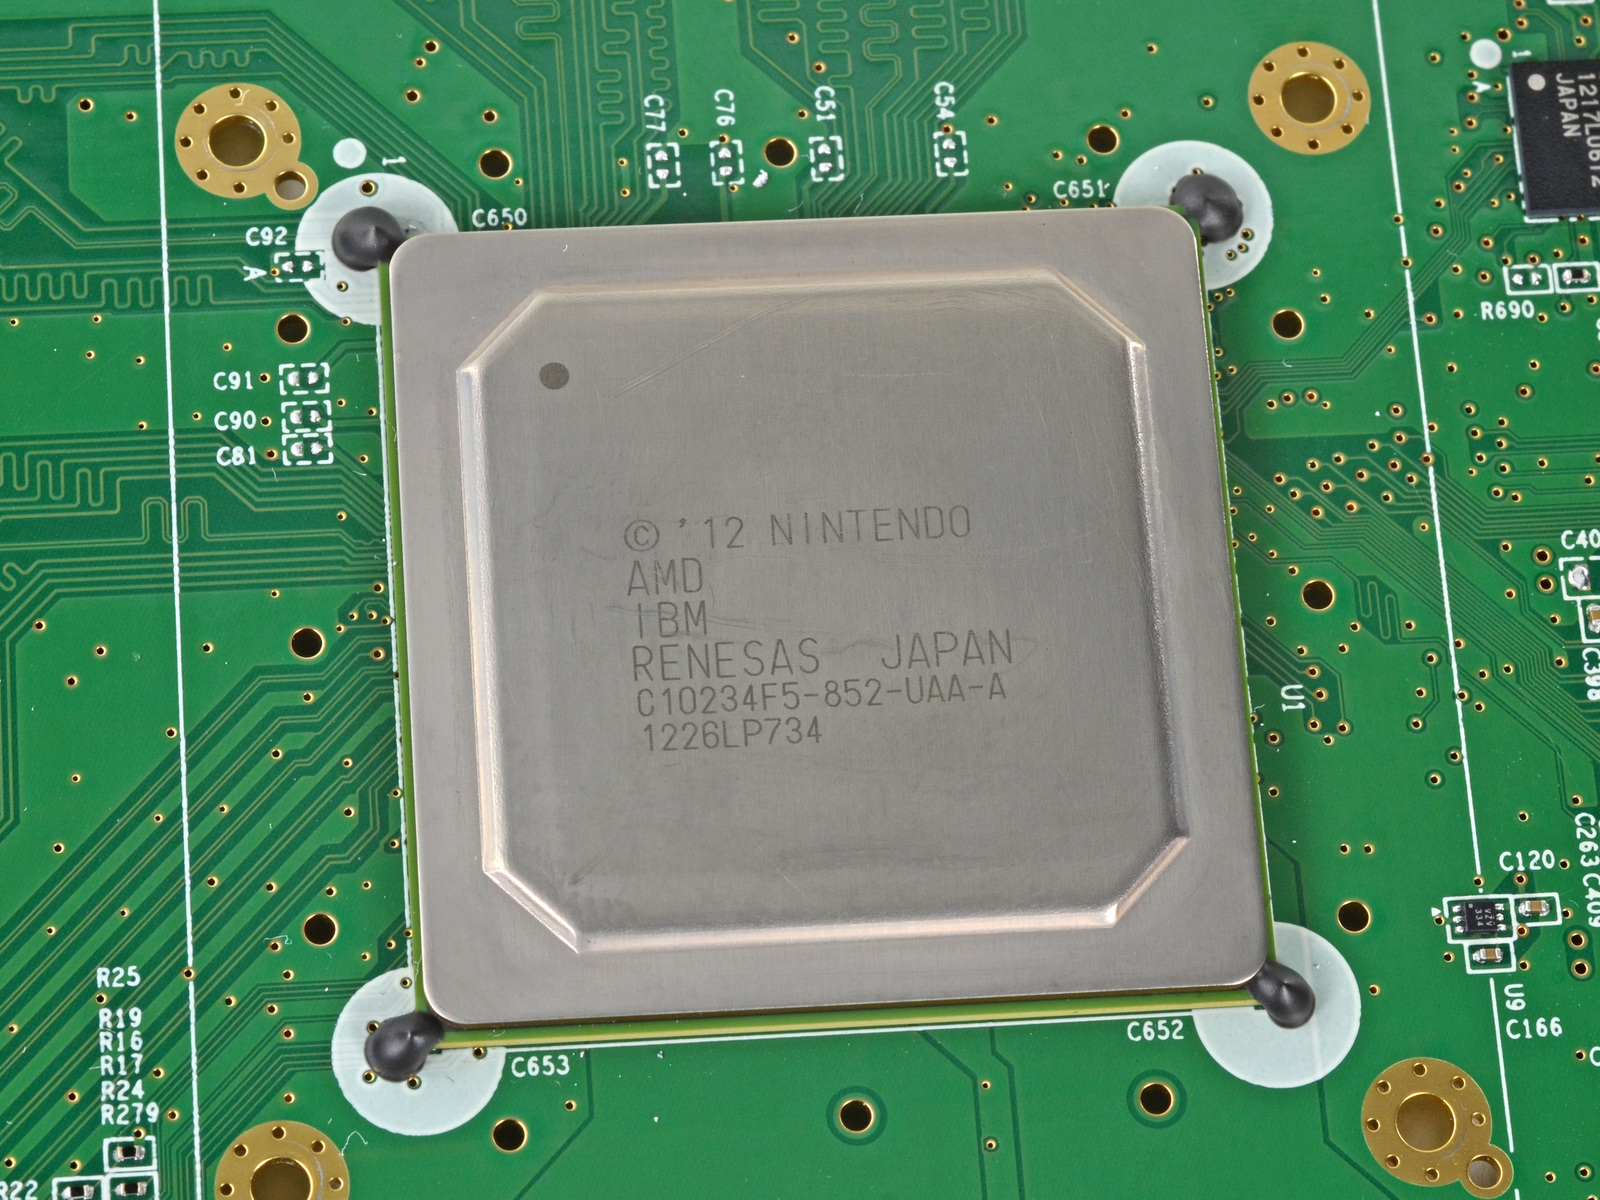
\includegraphics[width=\textwidth]{CPU_&_GPU.png}
				\caption{Wii U Multi Chip Module}
				\label{fig:mcm}
			\end{minipage}
		\end{figure}
		\begin{figure}[ht]
			\centering
			\begin{minipage}{0.45\textwidth}
				\centering
				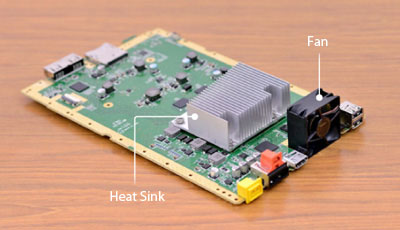
\includegraphics[width=\textwidth]{fan-heatsink.jpeg}
				\caption{Fan and heat sink position}
				\label{fig:fan-heatsink}
			\end{minipage}
			\hspace{0.5cm}
			\begin{minipage}{0.45\textwidth}
				\centering
				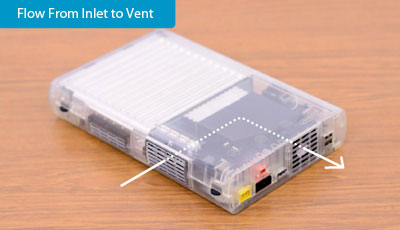
\includegraphics[width=\textwidth]{air_flow.jpeg}
				\caption{Wii U air flow demonstration}
				\label{fig:airflow}
			\end{minipage}
		\end{figure}

		In \autoref{fig:external} is shown the console without its external case.
		The first thing we note is that the bigger components inside the Wii U are the optical drive, a single heat sink used to cool down the entire console and two fans to allow the air to pass through the console.

		Analysing the position of the fans and of the heat sink, we note that the heat sink is over the main source of heat (CPU and GPU) and it is close to the fan rotated in a way that the air can pass through it, as shown in \autoref{fig:airflow}.

		Removing the heat sink we see another thermal compound that cover both CPU and GPU. These two are put close each other to reduce the latency and power consumption.

	\subsection{GamePad}
		The GamePad transformer has a maximum output voltage of 4.75V and a maximum output current of 1.6A, so it consumes $4.75\cdot 1.6 = 7.6W$ while under full load.
		\begin{figure}[htbp]
			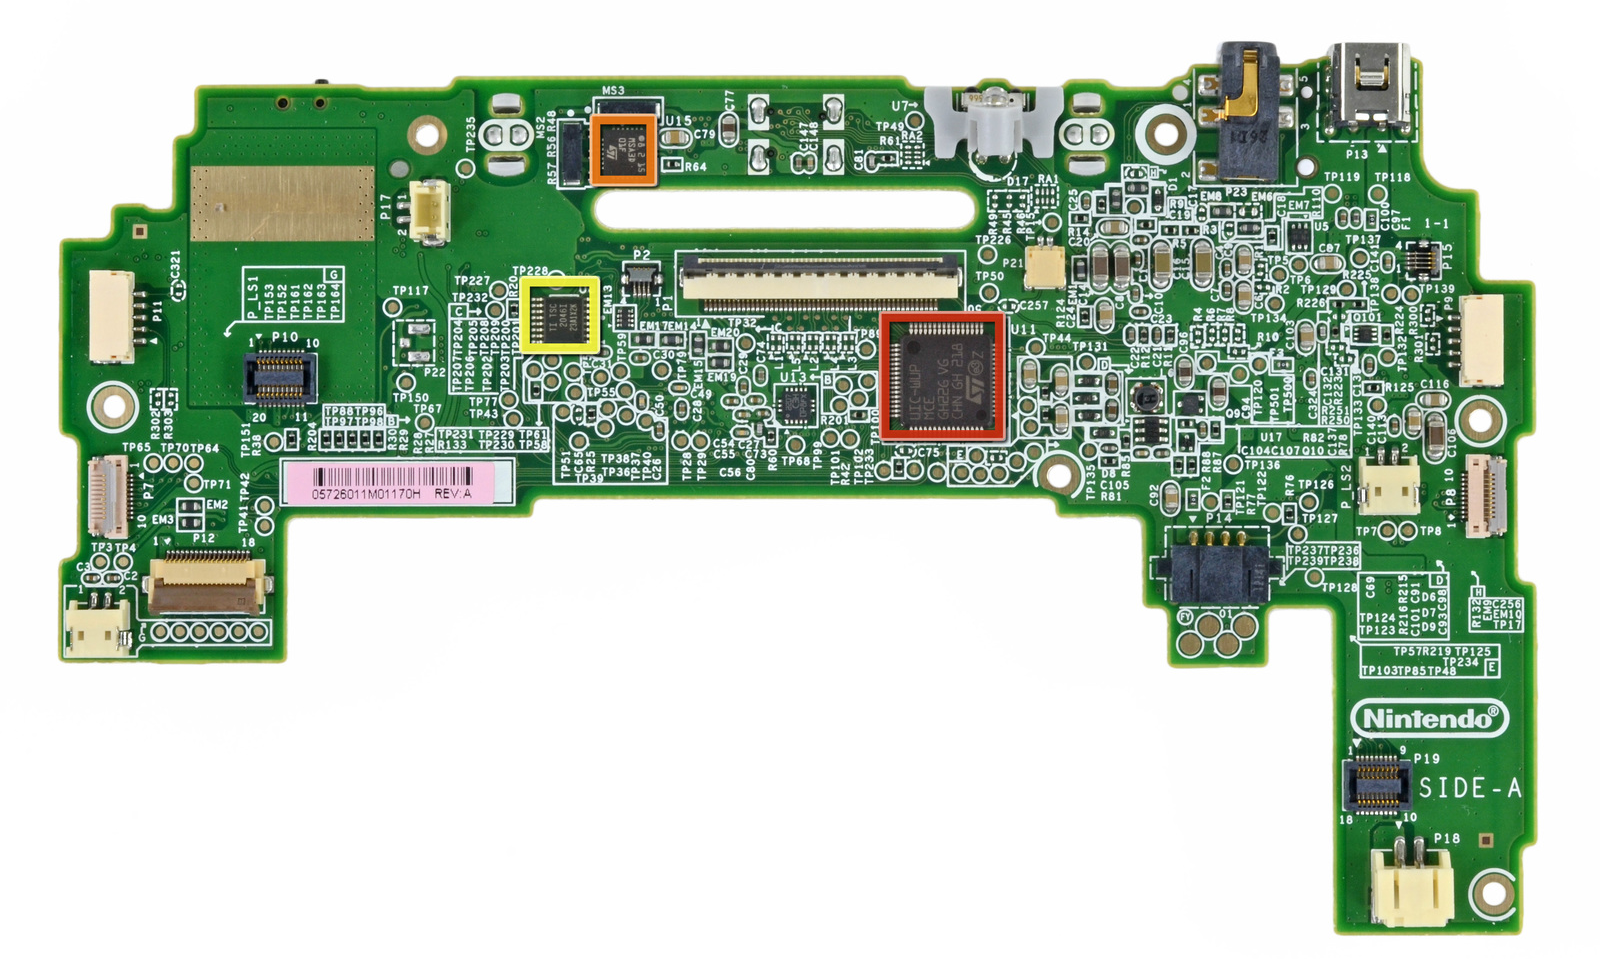
\includegraphics[width=\textwidth]{gamepad_motherboard_front.png}
			\caption{GamePad's motherboard}
			\label{fig:gamepad_motherboard}
		\end{figure}
		\subsubsection{Touch Screen Controller}
			TSC2046I is the touch screen controller used in the GamePad of the Wii U. TSC2046I is a chip integrated in the GamePad's motherboard, specifically is the chip in the yellow square in \autoref{fig:gamepad_motherboard}.

			Checking the datasheet \cite{touchscreen} we can get some interesting information.
			\begin{itemize}
				\item It has an on-chip $2.5V$ voltage reference that can be used for the auxiliary input, battery monitor, and temperature measurement modes. This can be powered down when not used to conserve power.
				\item The power consumption is less than $0.75mW$ at $2.7V$.
			\end{itemize}

			In \autoref{tab:thermal_touch} are summarized the parameters relatively to the thermal management of the chip.

			In \autoref{fig:vref_temp} and \autoref{fig:vref_vcc} is shown as the on-chip reference voltage previously mentioned is actually not fixed at $2.5V$ but is floating around this value and depends on the Temperature and on the input voltage $V_{CC}$. In \autoref{fig:sample_vcc} and \autoref{fig:vcc_temp} is shown as the Sample Rate of the Touch Screen Controller varies with the input voltage and how this last one varies with the temperature.

			In general we can deduct that if $V_{CC}$ is too low (more or less lower than $3V$), both the sample rate and the reference voltage $V_{REF}$ will decrease.


			\begin{table}[htbp]
				\centering
				\begin{tabular}{cc}
					\toprule
					Parameter & Value\\
					\midrule
					Power Dissipation		 & 250mW\\
					Maximum Junction Temperature  & $+150^\circ C$\\
					Operating Temperature Range & $-40^\circ C$ to $+85^\circ C$ \\
					Storage Temperature Range & $-65^\circ C$ to $+150^\circ C$ \\
					Lead Temperature  & $+300^\circ C$\\
					\bottomrule
				\end{tabular}
				\caption{Thermal management in TSC2046I}
				\label{tab:thermal_touch}
			\end{table}

			\begin{figure}[htbp]
				\begin{minipage}{.5\textwidth}
					\centering
					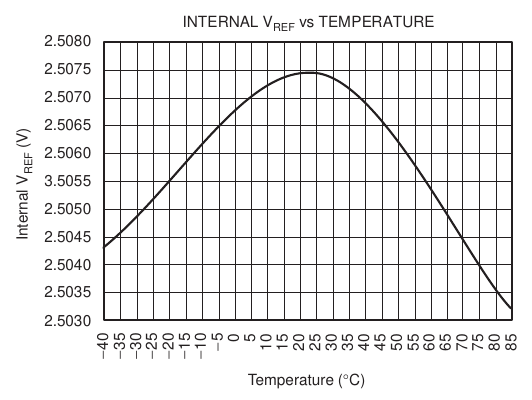
\includegraphics[width=\textwidth]{v_ref_temp.png}
					\caption{Variation of $V_{REF}$ with Temperature}
					\label{fig:vref_temp}
				\end{minipage}
				\begin{minipage}{.5\textwidth}
					\centering
					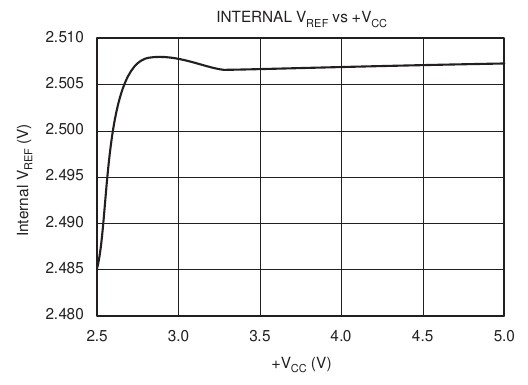
\includegraphics[width=\textwidth]{v_ref_vcc.png}
					\caption{Variation of $V_{REF}$ with $V_{CC}$}
					\label{fig:vref_vcc}
				\end{minipage}
			\end{figure}

			\begin{figure}[htbp]
				\begin{minipage}{.5\textwidth}
					\centering
					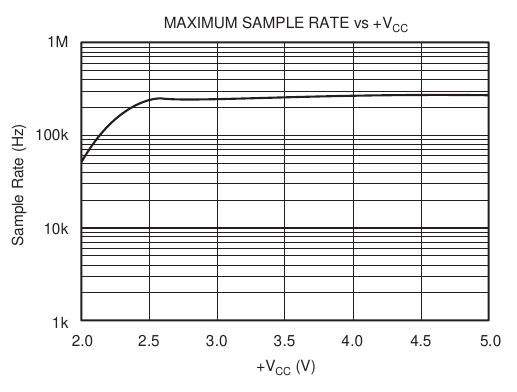
\includegraphics[width=\textwidth]{samplerate_vcc.png}
					\caption{Variation of the Sample Rate with $V_{CC}$}
					\label{fig:sample_vcc}
				\end{minipage}
				\begin{minipage}{.5\textwidth}
					\centering
					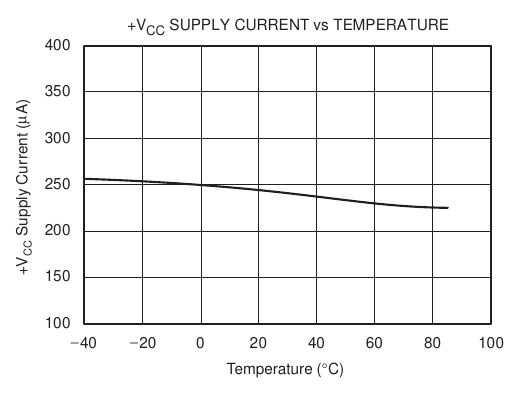
\includegraphics[width=\textwidth]{VCC_temp.png}
					\caption{Variation of $V_{CC}$ with the temperature}
					\label{fig:vcc_temp}
				\end{minipage}
			\end{figure}

			Finally, the temperature inside the chip is measured through a diode in the following way.
			The diode voltage $V_{BE}$ has a well-defined characteristic versus temperature, so the ambient temperature can be predicted in applications by knowing the +25°C value of the $V_{BE}$ voltage and then monitoring the delta of that voltage as the temperature changes.
			\newpage

		\subsubsection{Dual Antenna Wireless Module}
			\begin{figure}[htbp]
				\centering
				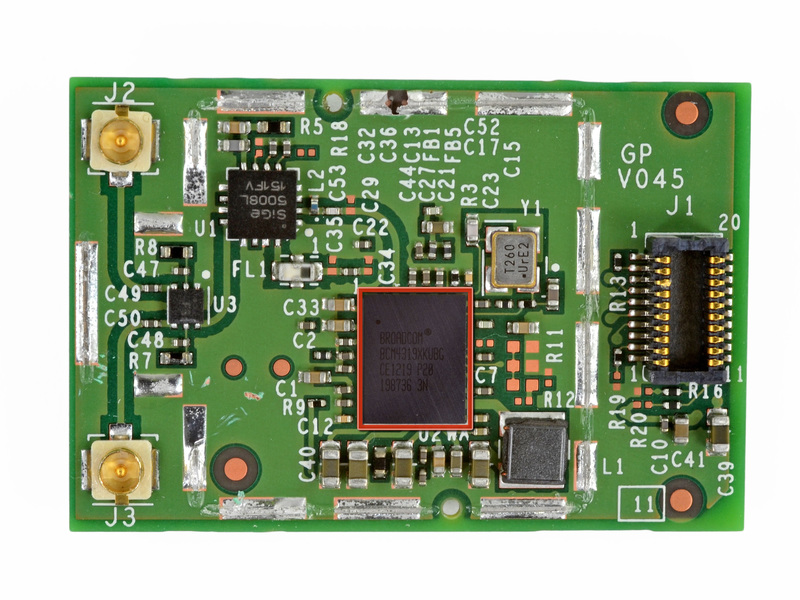
\includegraphics[width=.6\textwidth]{dual_antenna_wireless1.png}
				\caption{GamePad's wireless module}
				\label{fig:gamepad_wireless}
			\end{figure}
			Another module that can be extracted from the motherboard is the Dual Antenna Wireless Module, i.e. the module that allow to stream video and data between Wii U console and GamePad. It is shown in \autoref{fig:gamepad_wireless} and was mounted in place of the blue square in \autoref{fig:gamepad_motherboard}.

			This module is powered by a Broadcom BCM4319XKUBG (red square in \autoref{fig:gamepad_wireless}) and is explained in \cite{broadcom_wireless}.

			Its \gls{pmu} provides significant power savings by putting the BCM4319XKUBG into various power management states appropriate to the current environment and activities that are being performed. The \gls{pmu} enables and disables internal regulators, switches, and other blocks based on a computation of the required resources and the relationship between resources and the time needed to enable and disable them.

			Also the clock speed can be dynamically changed depending on the current requirements. Obviously, slower clock speeds are used wherever possible.

			Free different power states are defined:
			\begin{description}
				\item [Active Mode] All BCM4319XKUBG cores are powered up and fully functional. All required regulators are enabled and put in the most efficient mode.Clock speeds are dynamically adjusted by the \gls{pmu}.
				\item [Sleep Mode] All main clocks are shut down, only one clock is active and is used from the \gls{pmu} to wake up the chip. In Sleep mode, the primary power consumed is due to leakage current.
				\item	[Power-down mode] The BCM4319XKUBG is effectively powered off by shutting down all internal regulators. The chip is brought out of this mode by external logic re-enabling the internal regulators.

			\end{description}

\section{Electromagnetic compatibility}
  The console has also been designed in order to manage the electromagnetic compatibility of all its components. In particular, by observing the structure of the \gls{pcb}, we can notice several precautions regarding different aspects, like:
  \begin{itemize}
		\item Grounding;
		\item Shielding;
		\item Signal timing;
  \end{itemize}

  \subsection{Wii U main console motherboard PCB}
		\subsubsection{Grounding}
		  \begin{figure}[h]
				\begin{minipage}{.47 \textwidth}
				  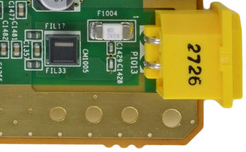
\includegraphics[width = .95\textwidth]{power_connector_top.png}
				  \caption{Power connector top side}
				  \label{fig:powertop}
				\end{minipage}
				\vspace{5mm}
				\begin{minipage}{.47 \textwidth}
				  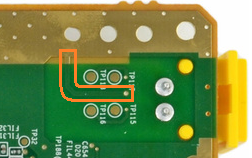
\includegraphics[width = .95\textwidth]{power_connector_bottom.png}
				  \caption{Power connector bottom side}
				  \label{fig:powerbottom}
				\end{minipage}
		  \end{figure}
		  The Wii U motherboard is a very complex entity and so in this work we will focus only on some examples of \gls{emc}. In \autoref{fig:powertop} and \autoref{fig:powerbottom} there are two zoomed images of the power connector and its relative components: from \autoref{fig:powertop} it can be seen the power and the ground connections as the two pins coming out from the connector and going to several capacitor. The lower pin represents the ground voltage reference, which is brought to the bottom side of the \gls{pcb} through the coupling capacitor n$\deg$ C1428. On the other hand, the fuse numbered as F1004, testifies that the upper pin is the power reference and it is coupled to the ground voltage through the capacitor n$\deg$ C1429. On the other figure (\autoref{fig:powerbottom}) we see the bottom side of the motherboard, where it is clear the connection of the top side voltage reference to the ground plane through the track framed in orange.

		  \begin{figure}[htbp]
					\centering
				  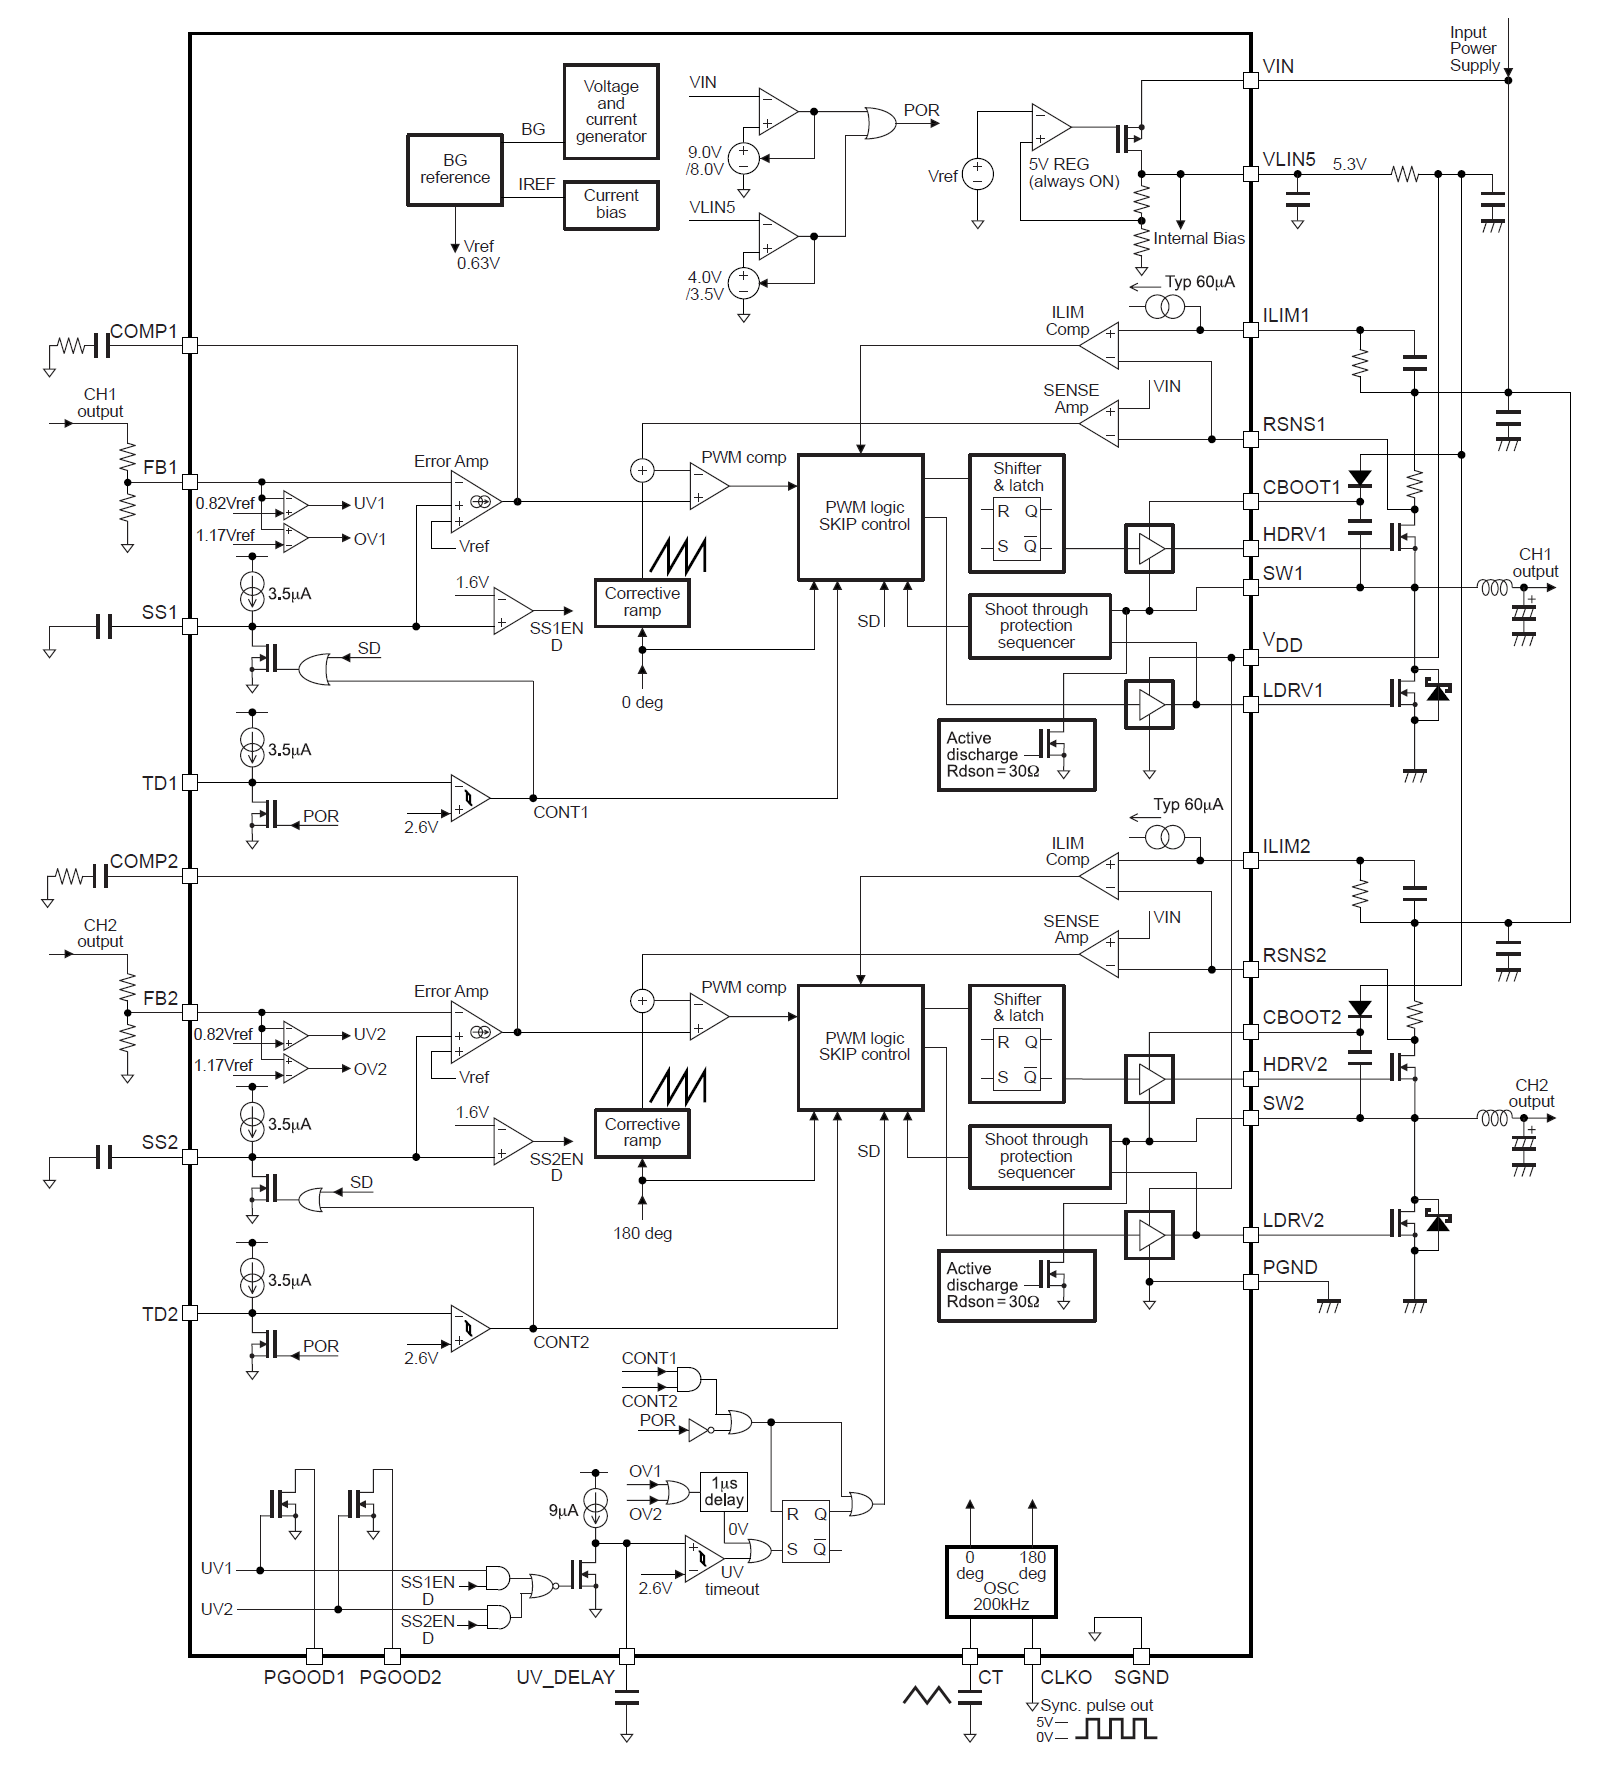
\includegraphics[width = \textwidth]{LV5065_block_diag.png}
				  \caption{LV065 Voltage controller block diagram}
				  \label{fig:LV5065bd}
			\end{figure}
		  \begin{figure}[htbp]
				\centering
				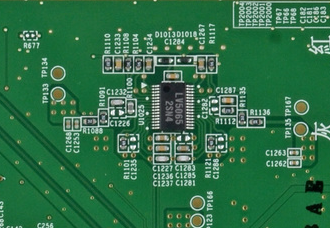
\includegraphics[width =.6\textwidth]{LV5065.png}
				\caption{LV065 Voltage controller}
				\label{fig:LV5065}
		  \end{figure}

		  Another example of grounding is represented in \autoref{fig:LV5065bd} and \autoref{fig:LV5065}, where there is a voltage regulator and its schematic. From the schematic we can see, for example, that some pins are part of the power structure of the \gls{ic} and are coupled with the ground level through some capacitor. In particular, pins $V_{IN}$ (number 15) and $V_{DD}$ (number 1) are connected to ground by two capacitors \DP{Dove è il numero dei pin in figura??}; moreover pins $VLIN5$, $V_{DD}$, $CBOOT1$ and $CBOOT2$ appear to be connected in a parallel way to ground. Finally, we can also see that pins $ILIM1$ and $ILIM2$ are connected to the same ground through the connection segment in green \DP{Quale segmento verde? La figura è in bianco e nero e nella foto in figura 21 non si vede il nome dei pin}, whose function is supposed to be avoiding quiet ground terminals and ground loops.

		  \subsubsection{Shielding}
				The motherboard is entirely enclosed in a metallic case in order to be well shielded, the case is shown in \autoref{fig:metalliccase}. Moreover, the aspect of shielding is present also in parts autonomous from the board, like cables going to the speakers or to the buttons (\autoref{fig:speaker} and \autoref{fig:button}): in this case we see the classic twisted cable useful to eliminate the constant component due to noise.

				\begin{figure}[h]
				  \begin{minipage}{.5 \textwidth}
						\centering
						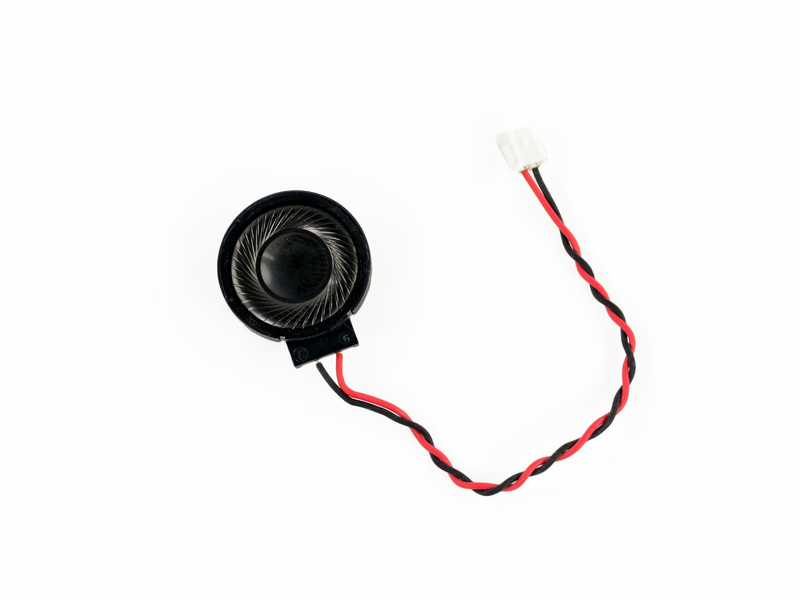
\includegraphics[width = \textwidth]{speaker.png}
						\caption{One of the console speakers}
						\label{fig:speaker}
				  \end{minipage}
				  \vspace{5mm}
				  \begin{minipage}{.5 \textwidth}
						\centering
						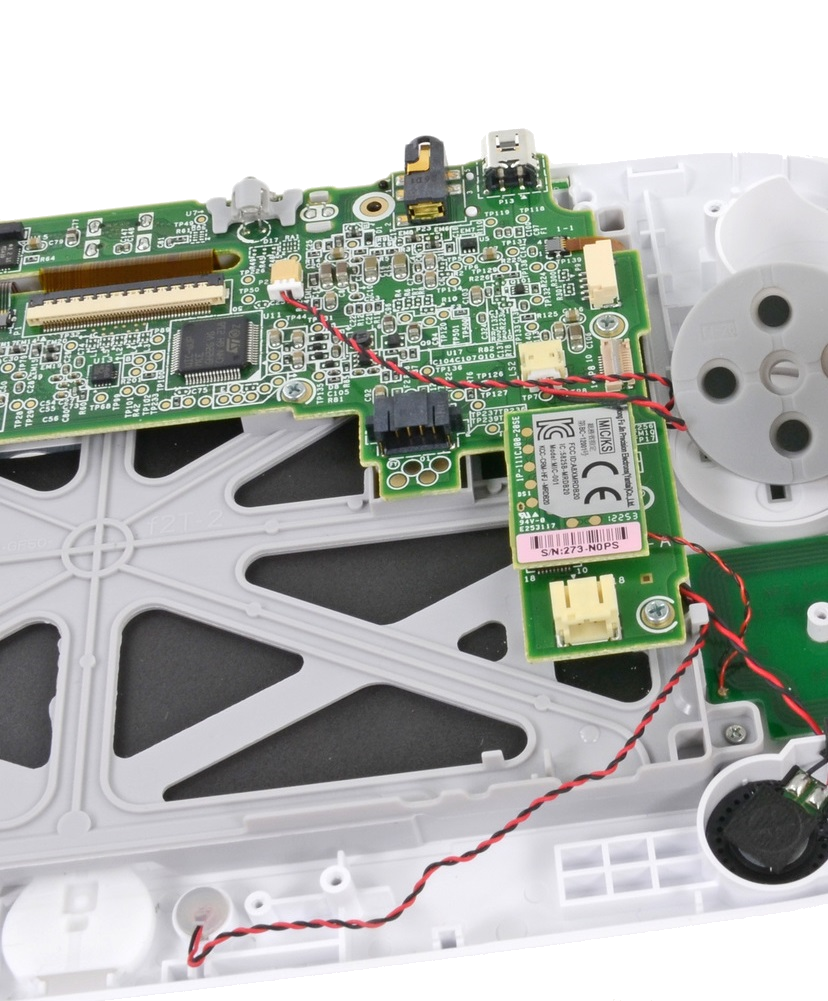
\includegraphics[width = .8\textwidth]{buttons.png}
						\caption{The connection to the console buttons}
						\label{fig:button}
				  \end{minipage}
				  \hspace{5mm}
				  \begin{minipage}{.5 \textwidth}
						\centering
						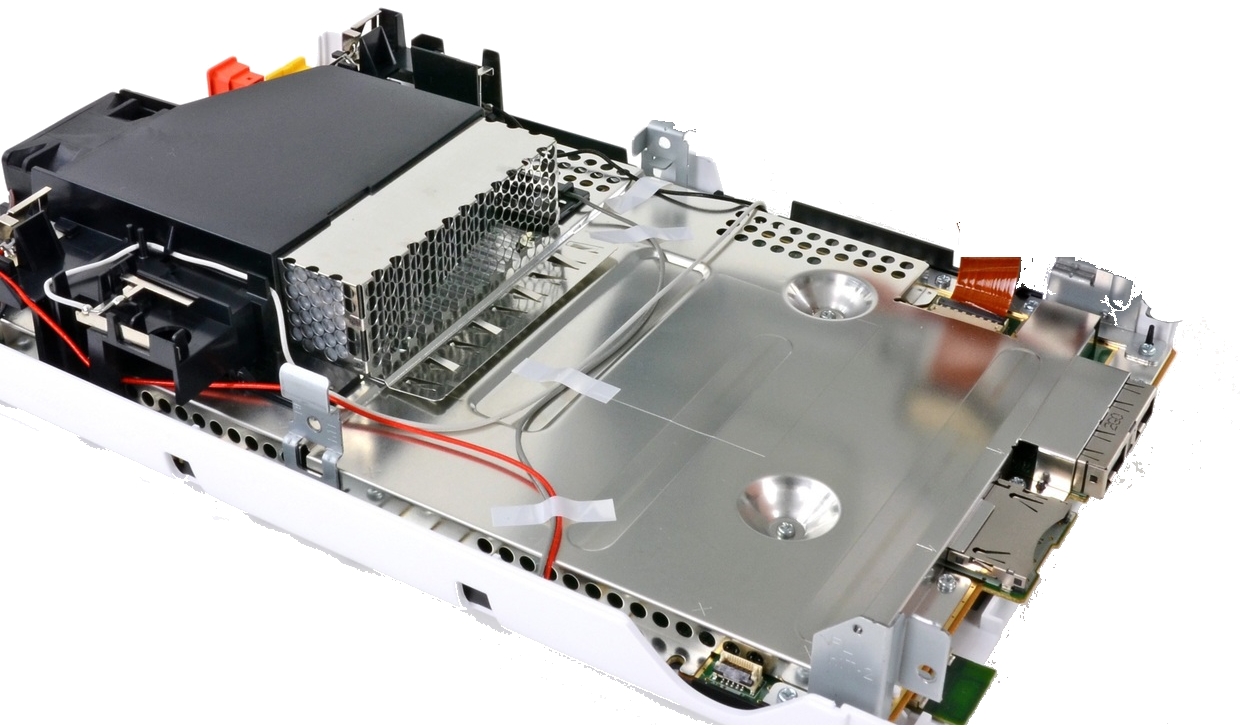
\includegraphics[width = .8\textwidth]{shield.png}
						\caption{The metallic case shielding the \gls{pcb}}
						\label{fig:metalliccase}
				  \end{minipage}
				\end{figure}

		  \subsubsection{General shrewdnesses}
				Other classical aspects characterize the design of this board:
				\begin{itemize}
				  \item as always, all the components and the tracks are surrounded by a ground plane useful to reduce coupling and radiation;
				  \item from \autoref{fig:motherboard} and \autoref{fig:motherboard_bottom} it can be observed the great amount of ground traces in between the shield;
				  \item the connectors of the board have several balancing resistances at the beginning/end of their transmission lines;
				  \item of course, all the components are \gls{smd} type in order to minimize the space and optimize the surface occupation of the pins, so as to reduce as much as possible the impedance of the pitches;
				  \item all the tracks have a width which is proportionate to the amount of current they have to bear, moreover there are no rect angles on them;
				\end{itemize}

				\begin{figure}[htbp]
				  \centering
				  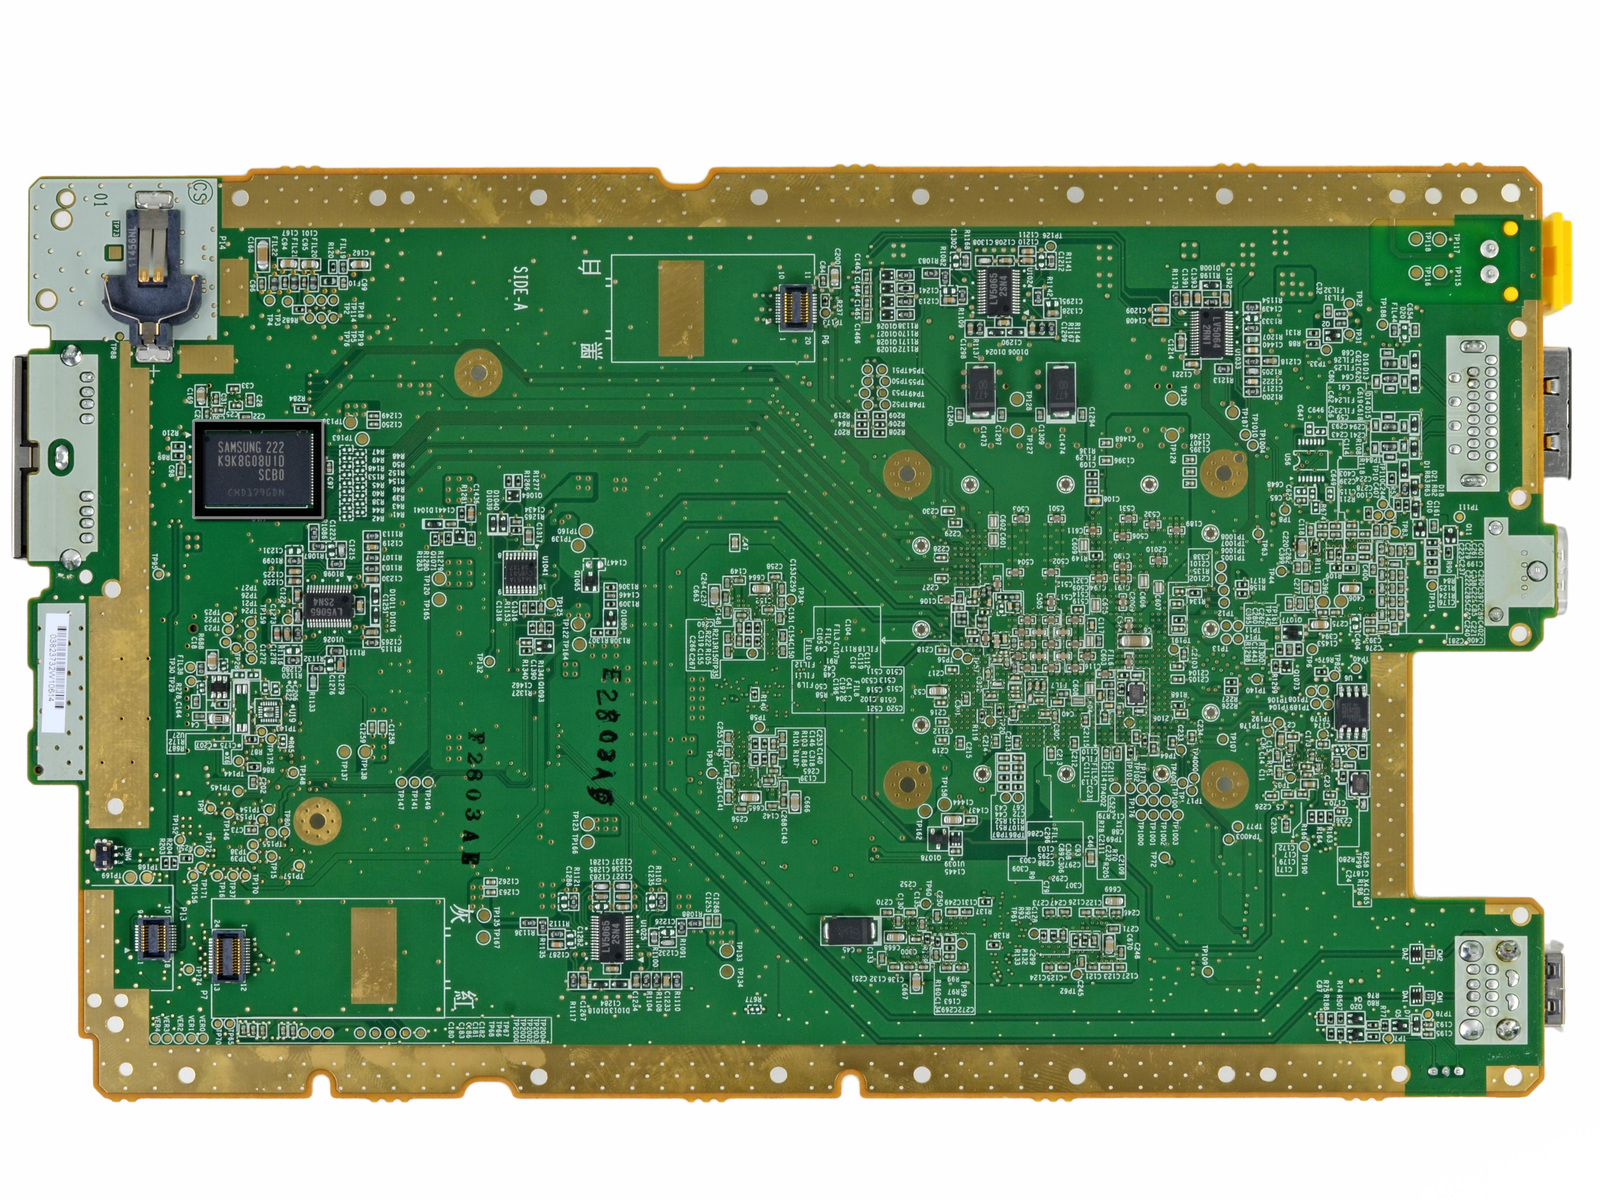
\includegraphics[width = .8\textwidth]{motherboard_back.png}
				  \caption{The bottom side of the motherboard \gls{pcb}}
				  \label{fig:motherboard_bottom}
				\end{figure}

	\section{Human Computer Interaction}
		\subsection{Wii U}
			Wii U has 4 USB ports (two more than its predecessor \textit{Wii}), and each of them allows also to recharge the GamePad. This allows the user to connect more devices such as External Hard Disks or USB pens containing photos, games or music.

			A failure in the Wii U design is that 2 GamePads are supported, but this feature has been never used since no games have been developed with the support to 2 GamePads.
		\subsection{GamePad}
			The first thing that the GamePad shows up when you try to connect it to your TV, is a brief questionary about your TV model.
			Indeed, with a dedicated button, Wii U's GamePad can control your TV, you can change the channel or the volume or you can view the program guide, as a normal Universal Remote.
			This interesting function makes sense in terms of efficiency since usually you use the Wii U in the same device where you normally watch the TV, so for a user is usual to switch between games and television, and having a single device to control everything makes this action simpler.

			Some months after the Wii U's release date, Nintendo released a service called \textit{TVii}, a platform that allows to use the GamePad as a Remote Controller for a cable TV (as the stock one yet explained) and for streaming platforms like \textit{Netflix}, \textit{Amazon Prime Video}, etc..
			The aim of the service is really functional to the device \DP{Non sono sicuro che si possa dire functional, volevo dire che l'aim di TVii è funzionale all'uso del GamePad}, but in the User Interface (the virtual one) 27 buttons at the same time are shown, plus 18 hard buttons distributed in the GamePad (in the front and in the back), making the usability of the service very difficult (the problem is shown in \autoref{fig:tviibuttons}).
			\begin{figure}[htbp]
				\begin{minipage}{.5\textwidth}
					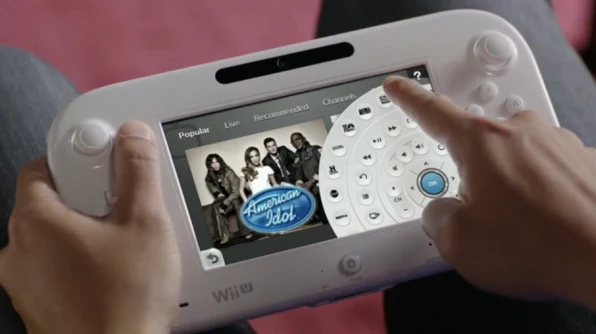
\includegraphics[width=\textwidth]{TViibuttons.png}
					\caption{TVii user interface}
					\label{fig:tviibuttons}
				\end{minipage}
				\begin{minipage}{.5\textwidth}
					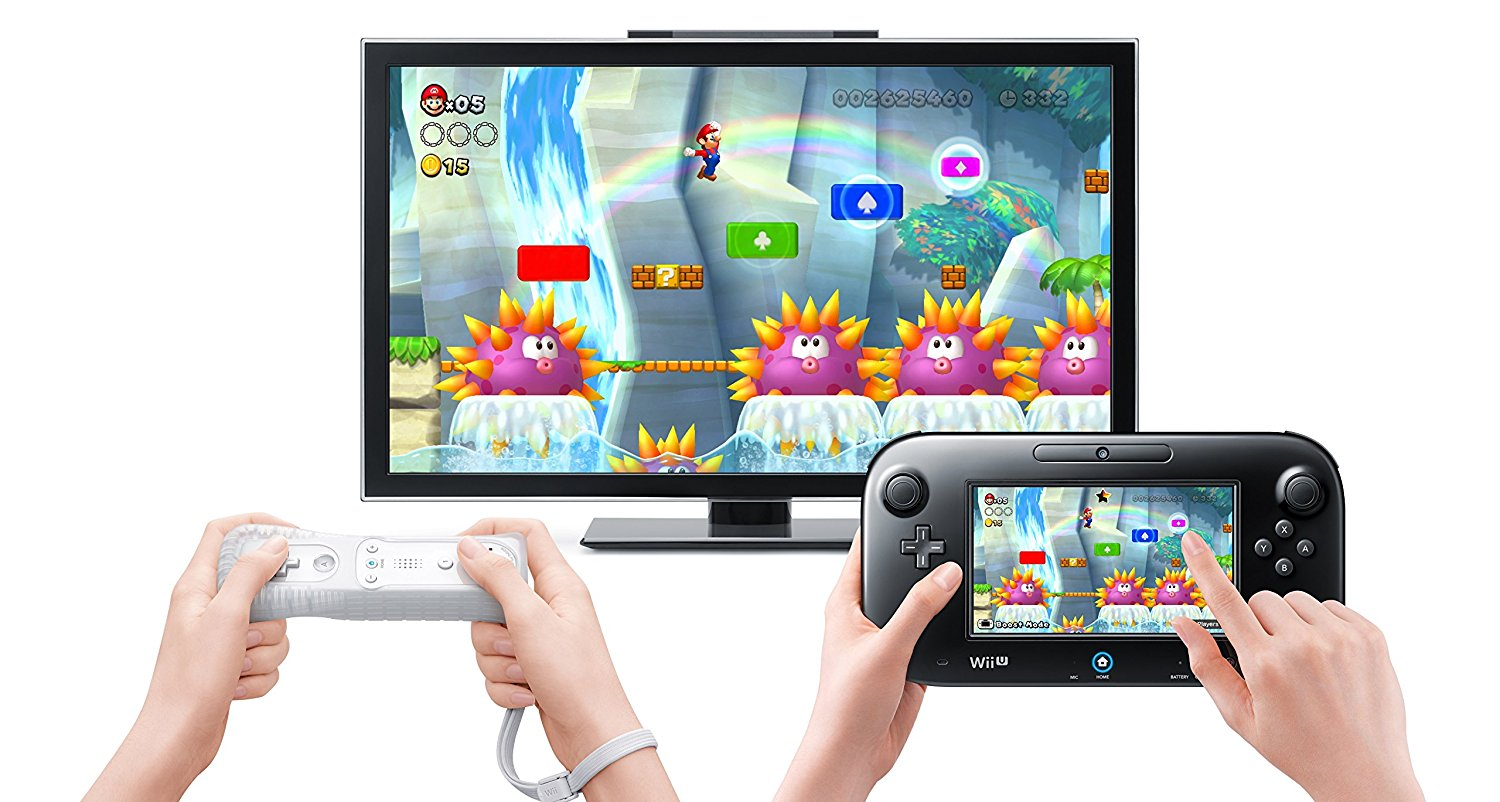
\includegraphics[width=\textwidth]{mariobrosu.jpeg}
					\caption{The TV screen mirrored in the GamePad makes the gameplay very confused}
					\label{fig:mariobros_u}
				\end{minipage}
			\end{figure}

			The GamePad offer four different input types:
			\begin{itemize}
				\item Hard buttons
				\item Touchscreen controller
				\item Stylus Pen
				\item Motion Control
			\end{itemize}
			This wide choice can be viewed as an innovative approach to this type of devices or, more probably, a confusing and not so comfortable feature.

			The possibility to have different type of inputs makes the videogames' design more complex, with the result that some games are developed to use most of Wii U's features, while the others use only a little part of them. Some games (even of the same \textit{Nintendo}), use the TV as a mirror for the GamePad, making the gameplay very confused.

			Another critical part in the Human Computer Interaction analysis is the battery life of the device.
			The device has an autonomy of (on average) 4 hours. Counting that the GamePad can be used both as Universal Remote or to play games, 4 hours are definetly not enough.

\bibliographystyle{IEEEtran}
\bibliography{IEEEabrv,bibliography}

\end{document}
